\chapter{\ifenglish Setup\else คู่มือการติดตั้ง\fi}


\begin{enumerate}
    \item Download file เกม Attention plaese for test.zip 
    \item[] สามารถดาวน์โหลดได้จาก \href{https://drive.google.com/drive/folders/1qNfmfBpqTUBqoQOXA6Qml4-LvWOseVcJ}{Download}
    \begin{center}
        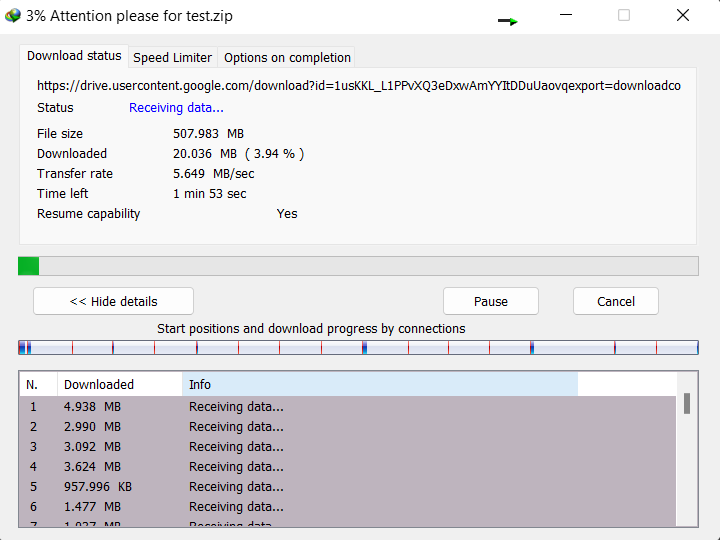
\includegraphics[width=1\textwidth, height=0.5\textheight]{Images/Download Image.png}
    \end{center}
    \item ทำการ Extract file เกม Attention please for test.zip ออกมา
    \begin{center}
        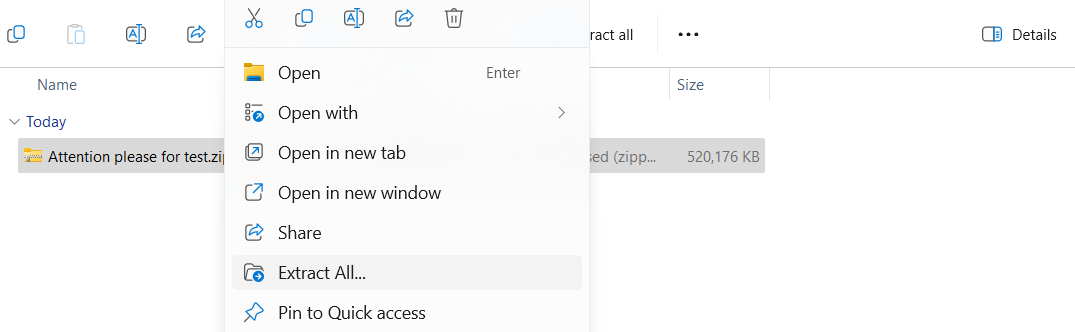
\includegraphics[width=1\textwidth, height=0.2\textheight]{Images/Extract Image.png}
    \end{center}
    \item เปิด folder: Attention please for test / Attention please for test ภายในจะพบกับ file เกม
    \begin{center}
        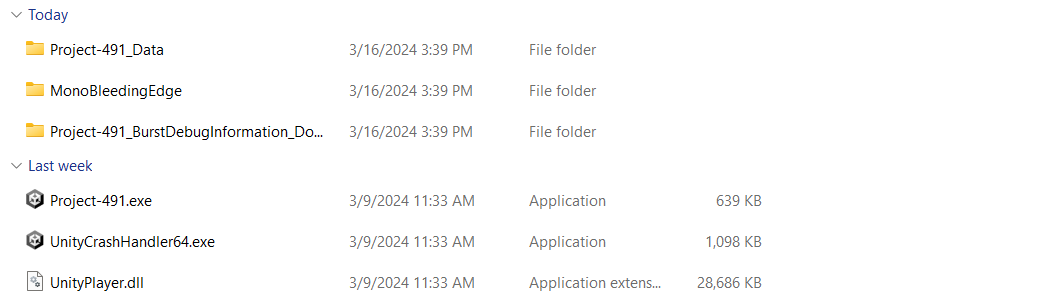
\includegraphics[width=1\textwidth, height=0.2\textheight]{Images/folder game.png}
    \end{center}
\end{enumerate}

% \section{Appendix section}

% Text for a section in the first appendix goes here.

% test ทดสอบฟอนต์ serif ภาษาไทย

% \textsf{test ทดสอบฟอนต์ sans serif ภาษาไทย}

% \verb+test ทดสอบฟอนต์ teletype ภาษาไทย+

% \texttt{test ทดสอบฟอนต์ teletype ภาษาไทย}

% \textbf{ตัวหนา serif ภาษาไทย \textsf{sans serif ภาษาไทย} \texttt{teletype ภาษาไทย}}

% \textit{ตัวเอียง serif ภาษาไทย \textsf{sans serif ภาษาไทย} \texttt{teletype ภาษาไทย}}

% \textbf{\textit{ตัวหนาเอียง serif ภาษาไทย \textsf{sans serif ภาษาไทย} \texttt{teletype ภาษาไทย}}}

% \url{https://www.example.com/test_ทดสอบ_url}

\chapter{\ifenglish Manual\else คู่มือการใช้งานระบบ\fi}

\section*{เริ่มต้นการใช้งาน}
\begin{enumerate}
    \item เมื่อกดเข้ามาในเกมครั้งแรก ผู้เล่นสามารถกดปุ่มเริ่มเกมเพื่อเริ่มต้นเกม
    \item หลังจากกดเข้ามาแล้ว ผู้เล่นจะต้องตั้งชื่อของตัวเอง จากนั้นกดยืนยัน
\end{enumerate}

\section*{การออกจากเกม}
\begin{enumerate}
    \item เมื่อผู้เล่นอยู่ที่หน้าเกมหลัก ผู้เล่นสามารถที่จะกดปุ่ม 
\includegraphics[width=0.05\textwidth, height=0.03\textheight]{Images/ExitBtn.png}
    \item เมื่อผู้เล่นอยู่ระหว่างทำการเล่นและต้องการที่จะออก ผู้เล่นสามารถกดปุ่ม Esc เพื่อทำการออกจากเกมได้
\end{enumerate}

\section*{การควบคุมตัวละครภายในเกม}
เมื่อผู้เล่นเข้ามา ผู้เล่นสามารถกดปุ่ม A D เพื่อที่จะทำให้ตัวละครเคลื่อนที่ไปทางซ้ายและทางขวา ตามลำดับ และผู้เล่นสามารถกดปุ่ม W S เพื่อขึ้นหรือลงบรรได
\begin{center}
    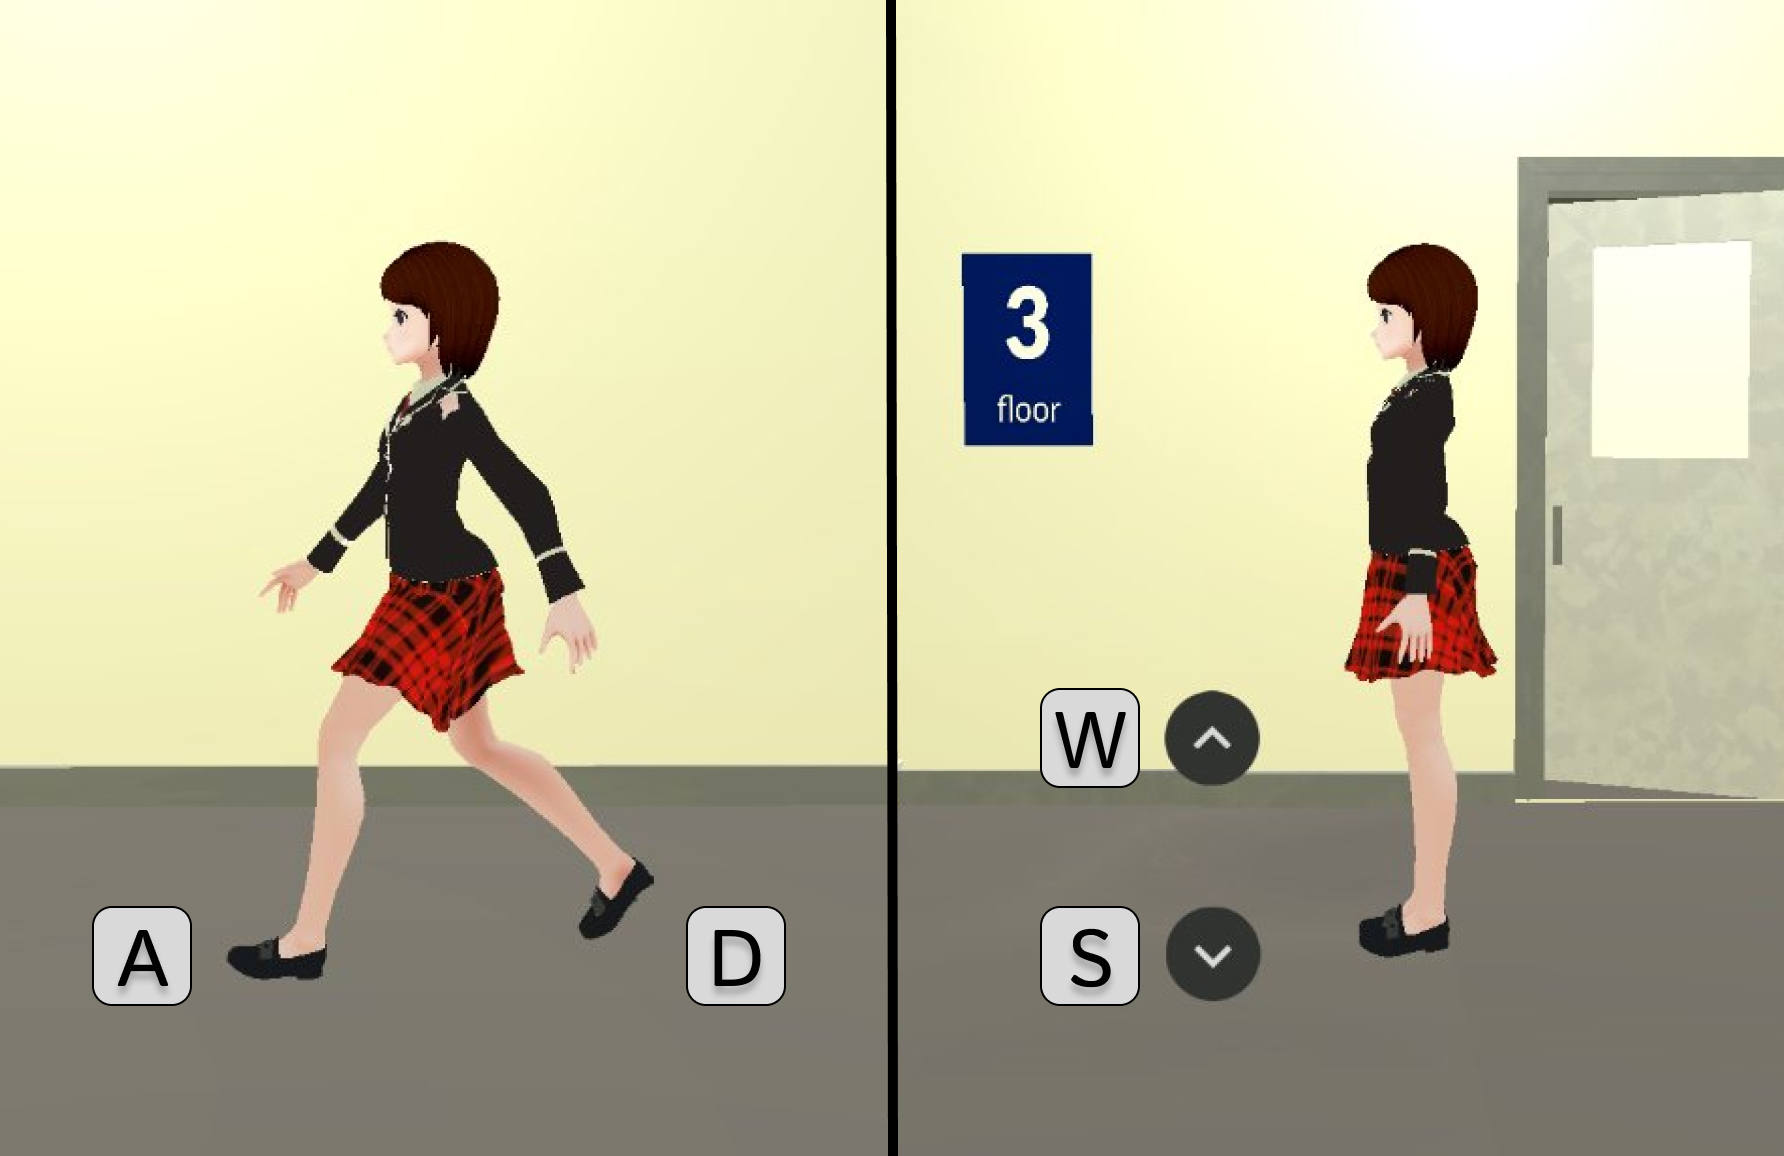
\includegraphics[width=0.7\textwidth, height=0.25\textheight]{Images/tutorial_move.png}
\end{center}

\section*{หน้า inventory ของเกม}
หน้า inventory จะแสดงเมื่อผู้เล่นกดปุ่ม I โดยจะมีให้เลือกการแสดงผลเป็นดังนี้
    \begin{enumerate}
        \item แถบสีแดง แสดงถึงพลังชีวิตของผู้เล่น
        \item ปุ่ม Food item
        \item ปุ่ม Question item
        \item ปุ่ม Task
        \item ปุ่ม Tutorial
    \end{enumerate}
    \begin{center}
        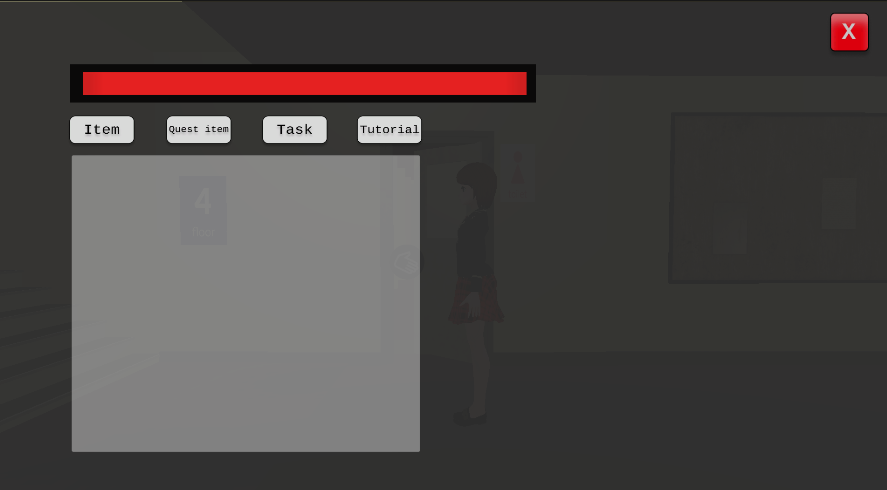
\includegraphics[width=0.8\textwidth, height=0.25\textheight]{Images/Inventory Image.png}
    \end{center}
\section*{การดำเนินเนื้อเรื่องภายในเกม}
ผู้เล่นจะได้สวมบทบาทเป็นนักเรียน /* Not yet */

\section*{หน้า Tutorial}
ผู้เล่นกดปุ่ม I เพื่อเปิดหน้า Inventory จากนั้นกดปุ่ม Tutorial จะแสดงปุ่ม Tutorial ต่างๆ
\begin{center}
    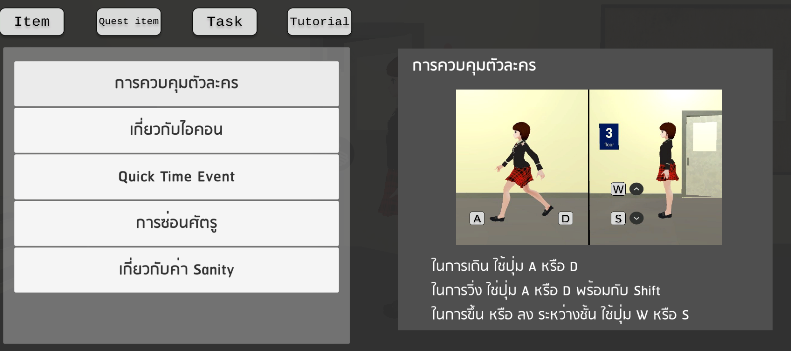
\includegraphics[width=0.8\textwidth, height=0.25\textheight]{Images/Tutorial Image.png}
\end{center}